\documentclass[11pt,a4paper]{article}

% =========================================================
% PAQUETES
% =========================================================
\usepackage[utf8]{inputenc}
\usepackage[T1]{fontenc}
\usepackage[spanish]{babel}
\usepackage{geometry}
\usepackage{graphicx}
\usepackage{booktabs}
\usepackage{array}
\usepackage{tabularx}
\usepackage{float}
\usepackage{hyperref}
\usepackage{setspace}

\geometry{
top=1.8cm,
bottom=1.8cm,
left=2cm,
right=2cm
}

\hypersetup{
colorlinks=true,
urlcolor=blue
}

\setlength{\parindent}{0pt}
\setlength{\parskip}{0.35em}
\setstretch{1.05}

% =========================================================
% DOCUMENTO
% =========================================================
\begin{document}

% =========================================================
% CARÁTULA
% =========================================================

\begin{titlepage}

\begin{center}

{\large \textbf{UNIVERSIDAD NACIONAL DE SAN ANTONIO ABAD DEL CUSCO}}

\vspace{0.4cm}

{\normalsize
\textbf{FACULTAD DE INGENIERÍA ELÉCTRICA, ELECTRÓNICA, INFORMÁTICA Y MECÁNICA}
}

\vspace{0.3cm}

{\normalsize
\textbf{ESCUELA PROFESIONAL DE INGENIERÍA INFORMÁTICA Y DE SISTEMAS}
}

\vspace{0.8cm}

% Logo UNSAAC

\includegraphics[width=4.3cm]{logo.png}

\vspace{1cm}

{\Large
\textbf{PRÁCTICA 02: TIPOS DE DATOS EN DART}
}

\vspace{0.5cm}

{\large
List, Map, Set y otros tipos de datos
}

\vspace{1.5cm}

\begin{flushleft}

\textbf{Alumno:} Héctor Paolo Barazorda Cuellar

\vspace{0.4cm}

\textbf{Docente:} Hans Harley Ccacyahuillca Bejar

\vspace{0.4cm}

\textbf{Curso:} DESARROLLO DE SOFTWARE II

\end{flushleft}

\vfill

{\large \textbf{Cusco -- Perú}}

\vspace{0.2cm}

{\large \textbf{2026}}

\end{center}

\end{titlepage}

% =========================================================
% SEGUNDA PÁGINA
% =========================================================

\section*{1. Objetivo}

Resolver los ejercicios de la guía sobre \texttt{List}, \texttt{Map} y
\texttt{Set}, demostrando además el uso de tipos primitivos, null safety,
records y \texttt{Runes} en Dart.

\section*{2. Ejercicios resueltos}

\begin{tabularx}{\textwidth}{>{\bfseries}p{2.7cm}X}
\toprule
Ejercicio & Solución implementada \\
\midrule
List & \texttt{mergeSortedLists} combina dos listas enlazadas ordenadas
reutilizando sus nodos. Complejidad: $O(n+m)$ en tiempo y $O(1)$ en espacio adicional. \\
Map & \texttt{intersectWithMultiplicity} cuenta las apariciones de los valores
con un mapa y consume cada coincidencia. Complejidad: $O(n+m)$. \\
Set & \texttt{countUnplacedFruitTypes} registra en un conjunto los índices de
cestas ocupadas y selecciona la primera cesta disponible suficiente. Complejidad: $O(n^2)$. \\
\bottomrule
\end{tabularx}

\section*{3. Tipos demostrados}

El programa también muestra tipos primitivos (\texttt{int}, \texttt{double},
\texttt{String}, \texttt{bool}, \texttt{dynamic} y \texttt{var}), null safety,
operaciones de listas, mapas y conjuntos, además de records y Unicode mediante
\texttt{Runes}.

\section*{4. Verificación}

Se ejecutaron los siguientes comandos:

\begin{verbatim}
dart analyze
dart run test/guide02_test.dart
dart run bin/main.dart
\end{verbatim}

El análisis no reportó problemas y todas las pruebas de los ejemplos de la
guía fueron aprobadas.

\section*{5. Enlaces de entrega}

\textbf{Repositorio GitHub:}
\url{https://github.com/hectorDev2/practica-02-dart}

\textbf{DartPad:}
\url{https://dartpad.dev/?id=40f1337e98900f5eb381175cdfb21fd6\&run=true}

\section*{6. Captura de respaldo}

La siguiente captura documenta la salida reproducible de la ejecución de
\texttt{bin/main.dart}:

\begin{figure}[H]
\centering
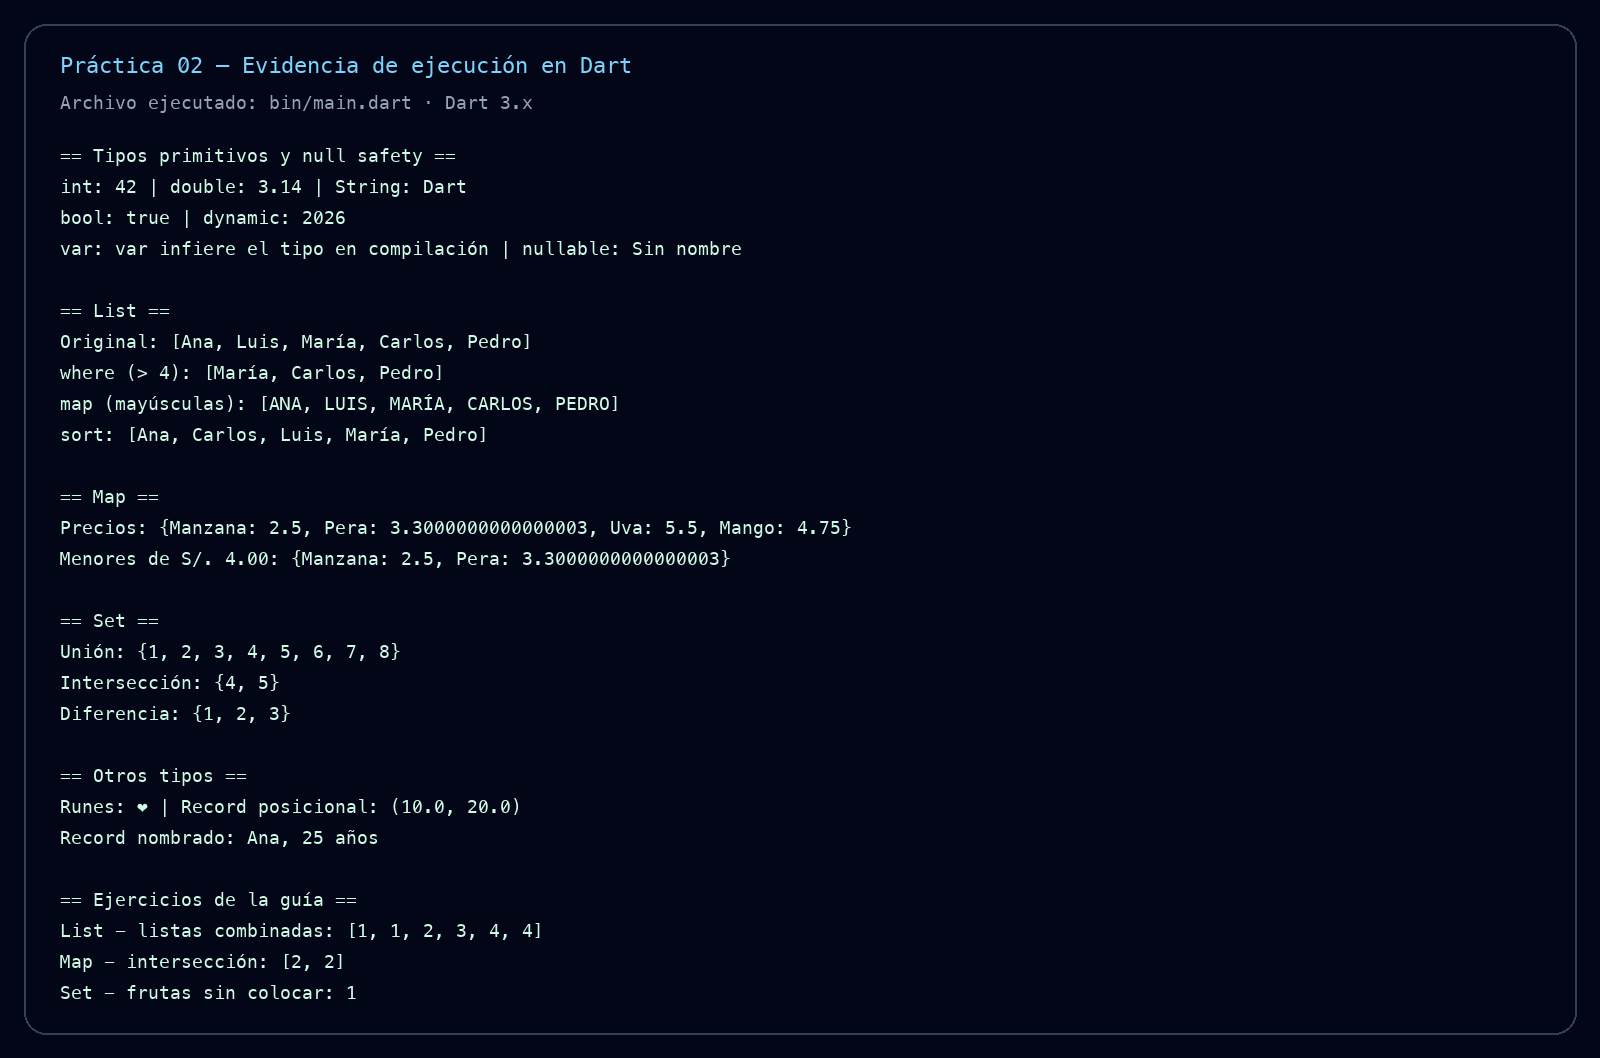
\includegraphics[width=\textwidth]{captura-ejecucion.png}
\caption{Evidencia de ejecución de la solución en Dart.}
\end{figure}

\end{document}
